\chapter{Un caso di studio: L'Abruzzo}
\label{ch:casodistudio}

Il focus del presente studio è posto, come è stato già preannunciato in precedenza, unicamente sulla regione Abruzzo, la cui rete ferroviaria, nonostante non abbia una estensione considerevole, è immersa in un territorio eterogeneo ed esposto a diversi livelli di rischio di natura idrogeologica. La ridotta estensione dei dati in esame, ha consentito di focalizzarsi su una analisi puntuale e non dispersiva dei metodi proposti, al fine di valutarne accuratamente la validità ed i limiti. Il presente \textit{report} è stato prodotto a fronte di un lavoro di laboratorio volto alla costruzione dei seguenti dati:
\begin{itemize}
\item  Una classifica delle stazioni, in base al potenziale rischio idrogeologico a cui esse sono esposte;
\item  Una classifica dei tratti di ferrovia maggiormente esposti a rischio di smottamenti del terreno su cui sono posti i binari.
\end{itemize}{}
La produzione di tali classifiche ha l’obiettivo di consentire una fruibilità facile ed immediata dei dati per quegli enti preposti al monitoraggio e alla manutenzione delle tratte e stazioni ferroviarie.
\newline
Di seguito si mostrerà una breve istantanea della attuale situazione osservata nel territorio abruzzese, con particolare attenzione ai dati selezionati, tra quelli disponibili, e alla loro provenienza.
\section{Territorio}
L'Abruzzo (rappresentata in fig.\ref{fig:regioneAbruzzo}) è una regione a statuto ordinario dell'Italia peninsulare, compresa tra il mare Adriatico e l'Appennino centrale,con capoluogo L'Aquila. La regione è geograficamente ed economicamente parte dell'Italia centrale, mentre dal punto di vista storico e linguistico è inserita all'interno dell'Italia meridionale.
\newline
Occupa una superficie di 10.831 km² e ha una popolazione di 1.322.349 abitanti. È diviso in quattro province: L'Aquila, Chieti, Pescara e Teramo, e in 305 comuni. Confina a nord con le Marche, ad est con il mare Adriatico, ad ovest con il Lazio e a sud con il Molise. Si divide principalmente in una parte costiera nel versante orientale con le spiagge dell'Adriatico, e in una parte montuosa dal lato occidentale con il Gran Sasso d'Italia (2.914 m s.l.m.), la Majella (2.793 m s.l.m.) e il Sirente-Velino (2.487 m s.l.m.) che costituiscono i tre massicci montuosi più alti dell'intera catena appenninica.
\newpage
\begin{figure}[bht]
	\centering
	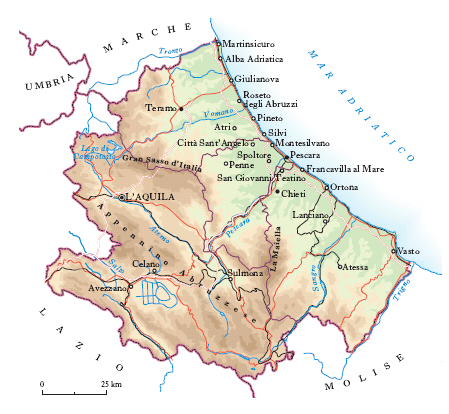
\includegraphics[width=0.4\textwidth]{img/regione}
	\caption{La regione Abruzzo}
    \label{fig:regioneAbruzzo}
\end{figure}

\section{Rete Ferroviaria}
Per quanto riguarda il trasporto ferroviario, vi è in Abruzzo una forte disparità tra quello moderno sulla costa (anche se con numero e qualità delle corse e del servizio imparagonabili rispetto all'asse ferroviario "tirrenico" e non è prevista alcuna linea di TAV) e quello delle zone interne, molto carente in termini di modernità e qualità del servizio e in attesa da decenni di interventi di potenziamento e ammodernamento (vedi in particolare la linea Pescara-Avezzano-Roma). Complessivamente comunque la rete ferroviaria abruzzese in attivo è abbastanza sviluppata e si estende per 524 km, mentre l'estensione totale complessiva della rete (attiva o dismessa) è pari a 648 km.

\subsection{Stazioni Ferroviarie}
I dati iniziali a nostra disposizione circa i nodi ferroviari ci forniscono le informazioni relative alle 114 stazioni distribuite sul territorio abruzzese mostrate in fig.\ref{fig:regioneStazione}.
\newpage
\begin{figure}[h]
	\centering
	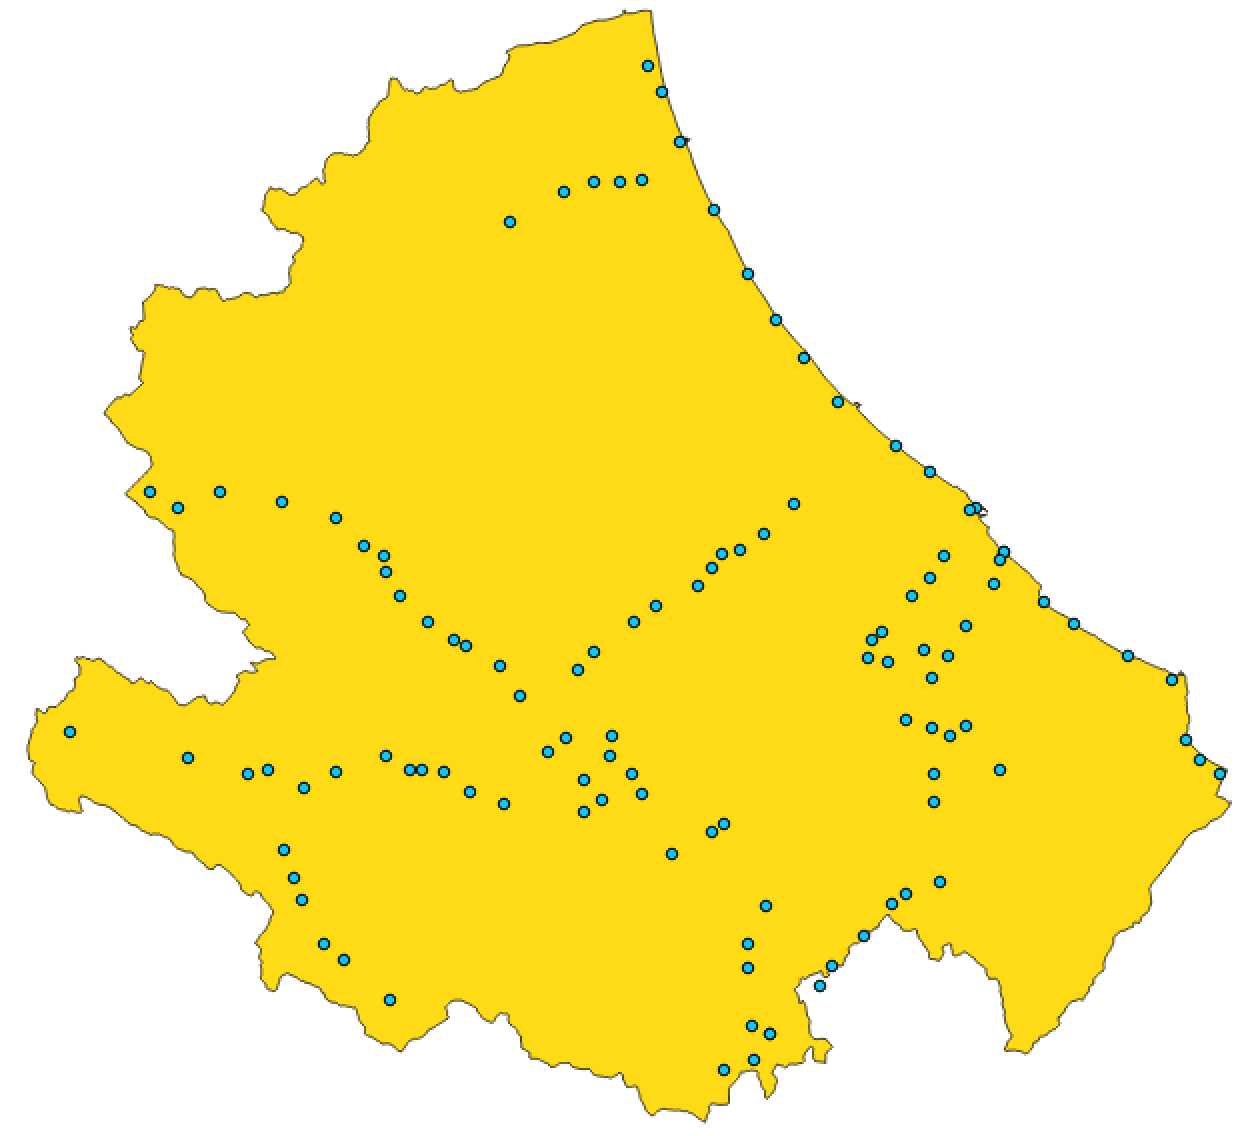
\includegraphics[width=0.4\textwidth]{img/regioneStazione}
	\caption{Stazioni ferroviarie presenti in Abruzzo}
    \label{fig:regioneStazione}
\end{figure}

\subsection{Linee Ferroviarie}
Sul territorio abruzzese sono presenti nove tratte ferroviarie:
\begin{itemize}
\item Bologna - Bari
\item Ortona - Crocetta
\item Marina di San Vito - Castel di Sangro
\item Roma - Pescara
\item Avezzano - Roccasecca
\item Archi stazione - Atessa
\item Sulmona - Carpinone
\item Rieti - L'Aquila - Sulmona
\item Teramo - Giulianova
\end{itemize}

\begin{figure}[h]
	\centering
	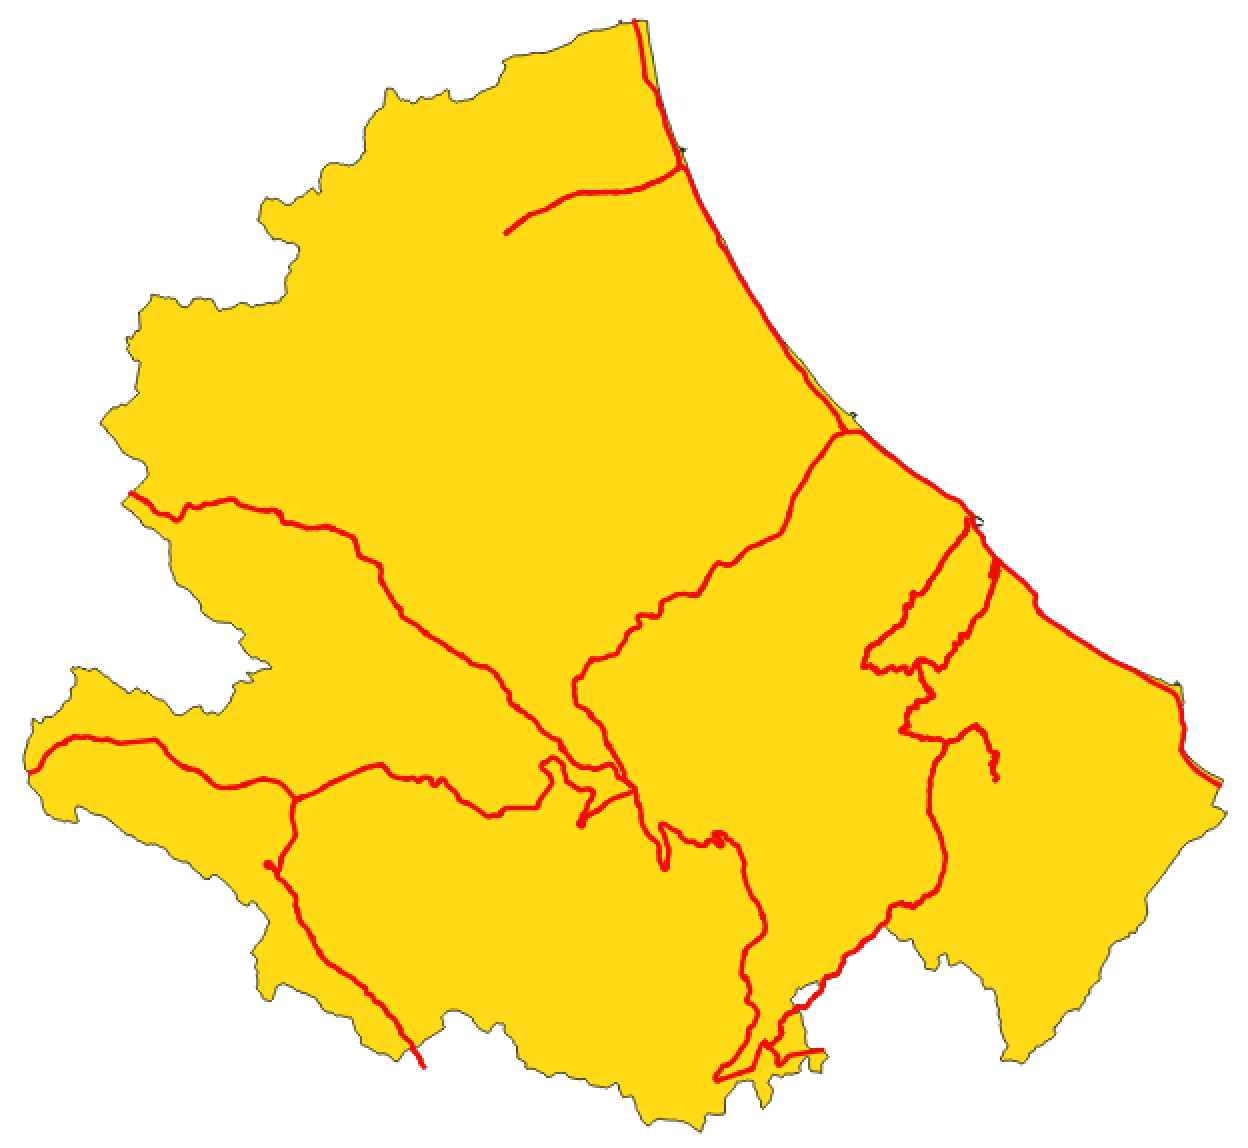
\includegraphics[width=0.4\textwidth]{img/regioneFerrovia}
	\caption{Linee ferroviarie presenti in Abruzzo}
    \label{fig:regioneFerrovia}
\end{figure}

Di queste tratte solo alcune sono completamente interne alla regione, altre invece la attraversano (avendo origine e/o fine al di fuori dei confini); riguardo queste ultime si è scelto di considerare unicamente le porzioni che cadono nella regione Abruzzo mostrate in fig.\ref{fig:regioneFerrovia}.
\newpage

\section{Zone}
\label{zone}
L'intero territorio abruzzese è stato completamente suddiviso in 22.000 zone più piccole la cui area media è pari a $0,5$ km$^2$. Il dataset relativo a queste zone ,che ci è stato fornito, è stato costruito mediante un algoritmo che segue un approccio basato sul \textit{diagramma di Voronoi}, tale da costruire una partizione completa del territorio determinata dalle distanze rispetto ad un determinato insieme discreto di elementi dello spazio (nel nostro caso un insieme finito di punti). Il risultato di tale partizionamento dello spazio è visibile nella Fig.\ref{fig:dataset}.
\begin{figure}[h]
	\centering
	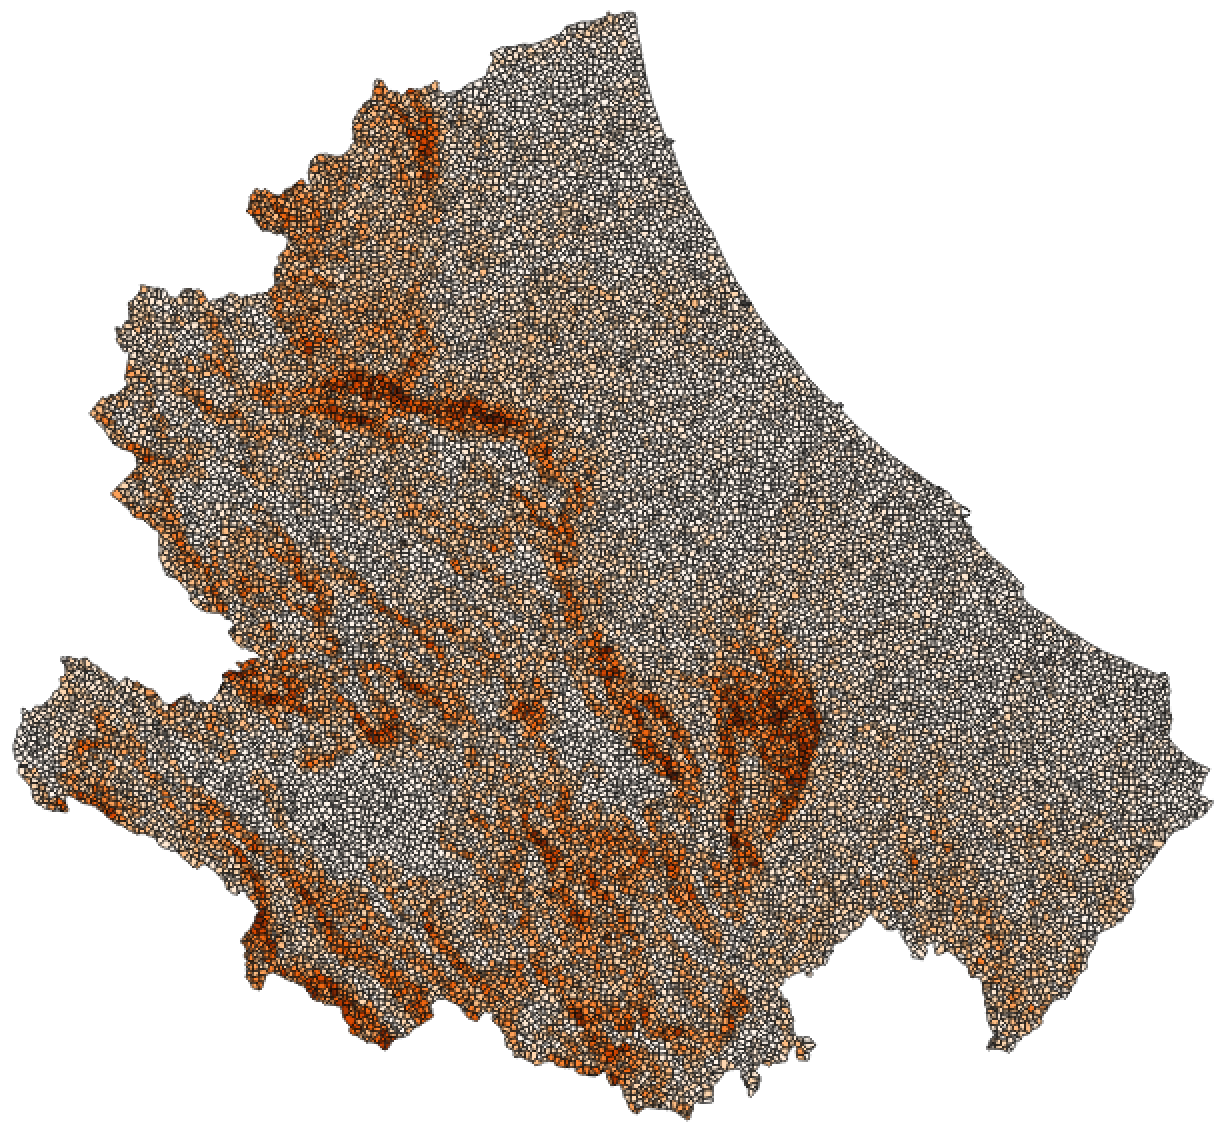
\includegraphics[width=0.5\textwidth]{img/dataset}
	\caption{Partizionamento completo della regione Abruzzo}
    \label{fig:dataset}
\end{figure}

Ad ogni $z_k$ è associato un valore numerico compreso tra $0$ e $1$, il quale quantifica la pericolosità determinata dal rischio idrogeologico della zona alla quale si riferisce.


%---------------
\section{Base di dati spaziale}
Si descrive in seguito la progettazione e conseguente realizzazione della base di dati geografica realizzata per un efficace implementazione degli algoritmi precedentemente descritti. Una base di dati spaziale accompagnata da un opportuno SGBD permette infatti di operare in modo agevole e naturale con dati geometrici, offrendo una gamma di operatori spaziali ottimizzati per la loro elaborazione. \\
I dati da memorizzare sono: 
\begin{itemize}
\item le stazioni e le linee ferroviarie abruzzesi con informazioni relative al nome e alla geometria;
\item la geometria dei confini dell'area geografica;
\item la geometria delle zone che vanno a partizionare in modo completo l'area con relative informazioni di rischio idrogeologico;
\item la geometria delle linee di livello presenti nel territorio di riferimento con la quota associata;
\item i risultati ottenuti dalle elaborazioni.
\end{itemize}

 

\subsection{Progettazione concettuale}
Per ogni entità verranno mostrate:

\begin{itemize}
\item gli attributi
\item l'attributo identificante
\item i vincoli di partecipazione nelle relazioni, con la notazione (min, max)
\end{itemize}

In Figura \ref{fig:er} si riporta il modello E-R della base di dati spaziale, mentre in Tabella \ref{tab:erTabellaEntita} sono elencate le entità con i relativi attributi, descrizione e attributi identificanti, ed infine in Tabella \ref{tab:erTabellaAssociazioni} l’elenco delle associazioni.
\pagebreak

\begin{figure}[h]
	\centering
	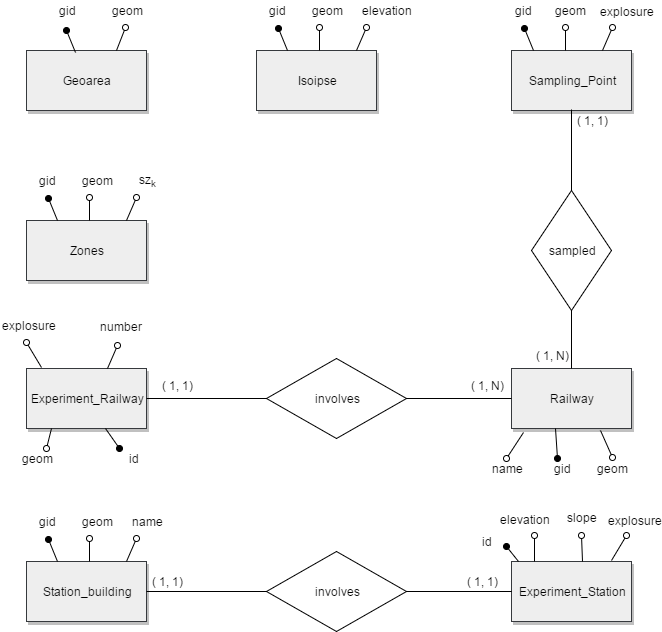
\includegraphics[width=1\textwidth]{img/er}
	\caption{Diagramma E-R della base di dati}
    \label{fig:er}
\end{figure}

Note:\\
l'attributo \textit{number} dell'entità \textit{Experiment\_railway}  rappresenta il numero del segmento relativo alla linea ferroviaria di appartenenza. Questo valore non è identificativo tra tutti i segmenti, ma solo tra i segmenti della linea al quale appartiene, quindi ad esempio su ogni linea sarà presente il segmento con \textit{number} pari ad uno.
\pagebreak

\begin{table}[h]
\centering
\begin{tabular}{|c|c|c|c|}
\hline
\textbf{Entità} & \textbf{Descrizione} & $\mathbf{Attributi}$ & \textbf{ID} \\
\hline

\multirow{3}{*}\textit{Geoarea} & Entità relativa al territorio di & \textit{gid} & \textit{gid}\\
& interesse. Nel nostro caso è la & \textit{geom} & \\&regione Abruzzo.&&\\ 
\hline

\multirow{3}{*}\textit{Zones} & Entità relativa al territorio di & \textit{gid} & \textit{gid}\\
& interesse. Nel nostro caso è un & \textit{sz$_k$} & \\
& partizionamento completo della &\textit{geom}& \\ 
& regione Abruzzo.&&\\ \hline

\multirow{3}{*}\textit{Station\_building} & Entità relativa alle stazioni & \textit{gid} & \textit{gid}\\
& presenti nel territorio di & \textit{name} & \\
& riferimento. &\textit{geom}& \\  \hline

\multirow{3}{*}\textit{Isoipse} & Entità relativa alle isoipse & \textit{gid} & \textit{gid}\\
& presenti nel territorio di & \textit{elevation} & \\
& riferimento. &\textit{geom}& \\  \hline

\multirow{3}{*}\textit{Railway} & Entità relativa alle linee ferroviarie & \textit{gid} & \textit{gid}\\
& presenti nel territorio di & \textit{name} & \\
& riferimento. &\textit{geom}& \\  \hline

\multirow{3}{*}\textit{Sampling\_point} & Entità relativa ai punti individuati & \textit{id} & \textit{id}\\
& come campionamento delle linee  & \textit{geom} & \\
&  ferroviarie presenti nel territorio &\textit{exposure}& \\
&  di riferimento. && \\  \hline

\multirow{4}{*}\textit{Experiment\_station} & Entità relativa agli esperimenti & \textit{id} & \textit{id}\\
& effettuati sulle stazioni & \textit{elevation} & \\
& presenti nel territorio& \textit{slope} & \\
& di riferimento. &\textit{exposure}& \\ \hline

\multirow{4}{*}\textit{Experiment\_railway} & Entità relativa agli esperimenti & \textit{id} & \textit{id}\\
& effettuati sulle linee ferroviarie  & \textit{geom} & \\
& presenti nel territorio &\textit{number}& \\
& di riferimento. & \textit{exposure}&\\ \hline

\end{tabular}
\caption{Tabella delle entità}
\label{tab:erTabellaEntita}
\end{table}

\begin{table}[h]
\centering
\begin{tabular}{|c|c|c|c|}
\hline
\textbf{Associazione} & \textbf{Descrizione} & $\mathbf{Entità\ coinvolte}$ & \textbf{Attributi} \\
\hline

\multirow{3}{*}\textit{involves} & Relazione che evidenzia il & \textit{station\_building} & \textit{nessuna}\\
& coinvolgimento di una sola & \textit{experiment\_station} & \\
& stazione in ogni esperimento. && \\ \hline

\multirow{3}{*}\textit{involves} & Relazione che evidenzia il  & \textit{railway} & \textit{nessuna}\\
& coinvolgimento di almeno una & \textit{experiment\_railway} & \\
& linea ferroviaria in uno o &&\\ 
& più esperimenti.&&\\
\hline

\multirow{3}{*}\textit{sampled} & Relazione che lega ogni linea & \textit{railway} & \textit{nessuna}\\
& ferroviaria con uno o più punti & \textit{sampling\_point} & \\
& di campionamento. &&\\ 
\hline

\end{tabular}
\caption{Tabella delle associazioni}
\label{tab:erTabellaAssociazioni}
\end{table}
\clearpage

\subsection{Progettazione logica}
Il diagramma E-R in figura \ref{fig:er} viene tradotto nello schema logico rappresentato graficamente in figura \ref{fig:schemaLogico}

\begin{figure}[h]
	\centering
	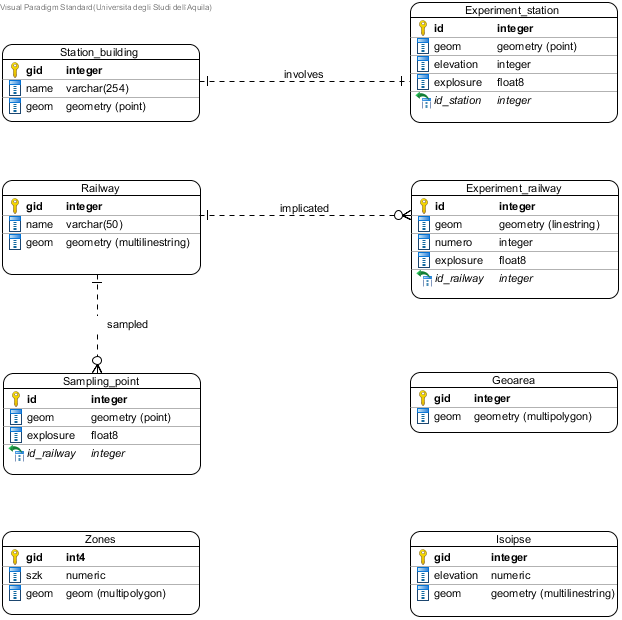
\includegraphics[width=1\textwidth]{img/schemaLogico}
	\caption{Schema logico}
    \label{fig:schemaLogico}
\end{figure}
